\chapter{Experimental Evaluation} \label{ch:experimental_evaluation}

In the following sections, all experiments conducted in order to resolve the research question in Section \ref{goals_and_research_questions} will be presented, and later used as a basis for discussion in the final section.









\section{Experimental Design}

From our testbed, we will be using \lstinline{pi3host2}, \lstinline{pi3host3} and \lstinline{pi3host4} as clients, with \lstinline{pi3host7} acting as a server. The clients will be sending bulk \gls{tcp} data over the bottleneck router \lstinline{pi3router} with a maximum bandwidth of \SI{10}{mbit} and a buffer size of 64 packets. To provide a fair share of the bandwidth for all flows during experiments, we will use the Fair Queuing version of \gls{codel} as the \gls{aqm} on the bottleneck router.









\section{Performance} \label{sec:performance}

In this section we will look at the performance of \gls{dabe} by comparing it directly against \gls{abe} and CUBIC. Each experiment will only have a single flow so it can freely use the available bandwidth. The resulting data will then be plotted against each other in order to draw comparisons. The \gls{teacup} configuration file can be found in Appendix \ref{app:teacup-performance}.


\subsection{Comparing Against ABE}

In this experiment we have run \gls{dabe} and \gls{abe} individually ten times each with four different delays on the bottleneck router. The following Figure \ref{fig:dabe_vs_abe_cwnd} shows the resulting \gls{cwnd} value over time for both \gls{dabe} and \gls{abe} taken from separate experiments.

\begin{figure}[H]
    \centering
    \includegraphics[width=1.0\linewidth]{performance2/dabe_vs_abe/cwnd}
    \captionsetup{width=1.0\linewidth}
    \caption{The \gls{cwnd} value for \gls{dabe} vs. \gls{abe} taken from separate experiments under various delays.}
    \label{fig:dabe_vs_abe_cwnd}
\end{figure}

Figure \ref{fig:dabe_vs_abe_rtt} shows the \gls{rtt} value over time for both \gls{dabe} and \gls{abe} taken from separate experiments.

\begin{figure}[H]
    \centering
    \includegraphics[width=1.0\linewidth]{performance2/dabe_vs_abe/rtt}
    \captionsetup{width=1.0\linewidth}
    \caption{The \gls{rtt} value for \gls{dabe} vs. \gls{abe} taken from separate experiments under various delays.}
    \label{fig:dabe_vs_abe_rtt}
\end{figure}

In order to assess the overall \gls{cwnd} and \gls{rtt} behavior for \gls{dabe} and \gls{abe}, the following Figure \ref{fig:dabe_vs_abe_avg} presents the average \gls{cwnd} and \gls{rtt} values from the ten runs that has been conducted.

\begin{figure}[H]
    \centering
    \begin{subfigure}{0.5\linewidth}
        \centering
        \includegraphics[width=1.0\linewidth]{performance2/dabe_vs_abe/cwnd_avg}
    \end{subfigure}%
    \begin{subfigure}{0.5\linewidth}
        \centering
        \includegraphics[width=1.0\linewidth]{performance2/dabe_vs_abe/rtt_avg}
    \end{subfigure}
    \caption{The average \gls{cwnd} and \gls{rtt} values for \gls{dabe} and \gls{abe}. The average is taken from running the experiment ten times.}
    \label{fig:dabe_vs_abe_avg}
\end{figure}

Figure \ref{fig:dabe_vs_abe_throughput} shows the throughput in four different delays for \gls{dabe} and \gls{abe}.

\begin{figure}[H]
    \centering
    \includegraphics[width=0.9\linewidth]{performance2/dabe_vs_abe/throughput}
    \captionsetup{width=0.9\linewidth}
    \caption{The throughput of \gls{dabe} and \gls{abe} under four different delays.}
    \label{fig:dabe_vs_abe_throughput}
\end{figure}









% \subsection{Comparing Against CUBIC}

% In this experiment we have run \gls{dabe} and CUBIC individually ten times each with four different delays on the bottleneck router. The following Figure \ref{fig:dabe_vs_cubic_rtt} shows the \gls{rtt} value over time for both \gls{dabe} and CUBIC taken from separate experiments.

% %The following Figure \ref{fig:dabe_vs_cubic_rtt} shows the resulting \gls{cwnd} value over time for both \gls{dabe} and CUBIC taken from separate experiments.

% % \begin{figure}[H]
% %     \centering
% %     \includegraphics[width=1.0\linewidth]{performance2/dabe_vs_abe/cwnd}
% %     \captionsetup{width=1.0\linewidth}
% %     \caption{The \gls{cwnd} value for \gls{dabe} vs. CUBIC taken from separate experiments under various delays.}
% %     \label{fig:dabe_vs_cubic_cwnd}
% % \end{figure}



% \begin{figure}[H]
%     \centering
%     \includegraphics[width=1.0\linewidth]{performance2/dabe_vs_CUBIC/rtt}
%     \captionsetup{width=1.0\linewidth}
%     \caption{The \gls{rtt} value for \gls{dabe} vs. CUBIC taken from separate experiments under various delays.}
%     \label{fig:dabe_vs_cubic_rtt}
% \end{figure}

% In order to assess the overall \gls{cwnd} and \gls{rtt} behavior for \gls{dabe} and CUBIC, the following Figure \ref{fig:dabe_vs_cubic_avg} presents the average \gls{cwnd} and \gls{rtt} values from the ten runs that has been conducted.

% \begin{figure}[H]
%     \centering
%     \begin{subfigure}{0.5\linewidth}
%         \centering
%         \includegraphics[width=1.0\linewidth]{performance2/dabe_vs_cubic/cwnd_avg}
%     \end{subfigure}%
%     \begin{subfigure}{0.5\linewidth}
%         \centering
%         \includegraphics[width=1.0\linewidth]{performance2/dabe_vs_cubic/rtt_avg}
%     \end{subfigure}
%     \caption{The average \gls{cwnd} and \gls{rtt} values for \gls{dabe} and CUBIC. The average is taken from running the experiment ten times.}
%     \label{fig:dabe_vs_cubic_avg}
% \end{figure}

% Figure \ref{fig:dabe_vs_cubic_throughput} shows the throughput in four different delays for \gls{dabe} and CUBIC.

% \begin{figure}[H]
%     \centering
%     \includegraphics[width=0.9\linewidth]{performance2/dabe_vs_cubic/throughput}
%     \captionsetup{width=0.9\linewidth}
%     \caption{The throughput of \gls{dabe} and CUBIC under four different delays.}
%     \label{fig:dabe_vs_cubic_throughput}
% \end{figure}








% \section{Single Flow}

% Figure \ref{fig:dabe_single_cwnd} \todo{...}

% \begin{figure}[H]
%     \centering
%     \includegraphics[width=1.0\linewidth]{performance/single_flow/cwnd}
%     \captionsetup{width=1.0\linewidth}
%     \caption{The \gls{cwnd} value of \gls{dabe} over time under various delays.}
%     \label{fig:dabe_single_cwnd}
% \end{figure}

% \begin{figure}[H]
%     \centering
%     \includegraphics[width=1.0\linewidth]{performance/single_flow/rtt}
%     \captionsetup{width=1.0\linewidth}
%     \caption{The \gls{rtt} value of \gls{dabe} over time under various delays.}
%     \label{fig:dabe_single_rtt}
% \end{figure}

% \begin{figure}[H]
%     \centering
%     \begin{subfigure}{0.5\linewidth}
%         \centering
%         \includegraphics[width=1.0\linewidth]{performance/single_flow/cwnd_avg}
%     \end{subfigure}%
%     \begin{subfigure}{0.5\linewidth}
%         \centering
%         \includegraphics[width=1.0\linewidth]{performance/single_flow/rtt_avg}
%     \end{subfigure}
%     \caption{\todo{update figure}}
% \end{figure}

% \begin{figure}[H]
%     \centering
%     \includegraphics[width=1.0\linewidth]{performance/single_flow/throughput}
%     \captionsetup{width=1.0\linewidth}
%     \caption{\todo{}}
%     %\label{fig:rtt_queue}
% \end{figure}









\section{Intra-Fairness} \label{sec:intra-fair}

In this section we will look at intra-fairness of \gls{dabe} by running experiments where it competes against itself.

\subsection{Two Flows}

In this section we have two flows of \gls{dabe} sharing the same link in order to see how they coexist with each other. The following Figure \ref{fig:dabe_vs_dabe_cwnd} shows the resulting \gls{cwnd} value over time when it competes against another \gls{dabe} flow.

\begin{figure}[H]
    \centering
    \includegraphics[width=1.0\linewidth]{performance/two_flows/cwnd}
    \captionsetup{width=1.0\linewidth}
    \caption{The \gls{cwnd} of \gls{dabe} when competing against another \gls{dabe} flow.}
    \label{fig:dabe_vs_dabe_cwnd}
\end{figure}

Figure \ref{fig:dabe_vs_dabe_rtt} shows the \gls{rtt} value over time when competing against another \gls{dabe} flow.

\begin{figure}[H]
    \centering
    \includegraphics[width=1.0\linewidth]{performance/two_flows/rtt}
    \captionsetup{width=1.0\linewidth}
    \caption{The \gls{rtt} of \gls{dabe} when competing against another \gls{dabe} flow.}
    \label{fig:dabe_vs_dabe_rtt}
\end{figure}

In order to assess the overall behavior when \gls{dabe} competes against another \gls{dabe} flow, the following Figure \ref{fig:dabe_vs_dabe_avg} presents the average \gls{cwnd} and \gls{rtt} values from ten experiments that has been conducted.

\begin{figure}[H]
    \centering
    \begin{subfigure}{0.5\linewidth}
        \centering
        \includegraphics[width=1.0\linewidth]{performance/two_flows/cwnd_avg}
    \end{subfigure}%
    \begin{subfigure}{0.5\linewidth}
        \centering
        \includegraphics[width=1.0\linewidth]{performance/two_flows/rtt_avg}
    \end{subfigure}
    \caption{The average \gls{cwnd} and \gls{rtt} when two flows of \gls{dabe} compete against each others. The average is taken from ten experiments.}
    \label{fig:dabe_vs_dabe_avg}
\end{figure}

Figure \ref{fig:dabe_vs_dabe_throughput} shows the throughput in four different delays when \gls{dabe} and \gls{abe} coexists.

\begin{figure}[H]
    \centering
    \includegraphics[width=1.0\linewidth]{performance/two_flows/throughput}
    \captionsetup{width=1.0\linewidth}
    \caption{The throughput of \gls{dabe} competing with another \gls{dabe} flow under four different delays.}
    \label{fig:dabe_vs_dabe_throughput}
\end{figure}









\subsection{Four Flows}

In this section we have four flows of \gls{dabe} sharing the same link in order to see how they coexist with each other. The following Figure \ref{fig:dabe_vs_dabe4_cwnd} shows the resulting \gls{cwnd} value over time when it competes against three other \gls{dabe} flows.

\begin{figure}[H]
    \centering
    \includegraphics[width=1.0\linewidth]{performance/four_flows/cwnd}
    \captionsetup{width=1.0\linewidth}
    \caption{The \gls{cwnd} of \gls{dabe} when competing against three other \gls{dabe} flows.}
    \label{fig:dabe_vs_dabe4_cwnd}
\end{figure}

Figure \ref{fig:dabe_vs_dabe4_rtt} shows the \gls{rtt} value over time when competing against three other \gls{dabe} flows.

\begin{figure}[H]
    \centering
    \includegraphics[width=1.0\linewidth]{performance/four_flows/rtt}
    \captionsetup{width=1.0\linewidth}
    \caption{The \gls{rtt} of \gls{dabe} when competing against three other \gls{dabe} flows.}
    \label{fig:dabe_vs_dabe4_rtt}
\end{figure}

In order to assess the overall behavior when \gls{dabe} competes against three other \gls{dabe} flows, the following Figure \ref{fig:dabe_vs_dabe4_avg} presents the average \gls{cwnd} and \gls{rtt} values from ten experiments that has been conducted.

\begin{figure}[H]
    \centering
    \begin{subfigure}{0.5\linewidth}
        \centering
        \includegraphics[width=1.0\linewidth]{performance/four_flows/cwnd_avg}
    \end{subfigure}%
    \begin{subfigure}{0.5\linewidth}
        \centering
        \includegraphics[width=1.0\linewidth]{performance/four_flows/rtt_avg}
    \end{subfigure}
    \caption{The average \gls{cwnd} and \gls{rtt} when four flows of \gls{dabe} compete against each others. The average is taken from ten experiments.}
    \label{fig:dabe_vs_dabe4_avg}
\end{figure}

Figure \ref{fig:dabe_vs_dabe4_throughput} shows the throughput in four different delays when four \gls{dabe} flows comepete against each other.

\begin{figure}[H]
    \centering
    \includegraphics[width=1.0\linewidth]{performance/four_flows/throughput}
    \captionsetup{width=1.0\linewidth}
    \caption{The throughput of four competing \gls{dabe} flows under four different delays.}
    \label{fig:dabe_vs_dabe4_throughput}
\end{figure}






\section{Mixed Flows} \label{sec:mixed-flows}

In this section we will look at how \gls{dabe} coexists with other flows. The \gls{teacup} configuration file for mixed flows can be found in Appendix \ref{app:teacup-mixed}.


\subsection{DABE and ABE}

In this experiment we have generated one flow using \gls{dabe} and another using \gls{abe} sharing the same link. Each experiment has been run ten times with four different delays. Figure \ref{fig:dabe_and_abe_cwnd} shows the \gls{cwnd} value over time with both flows present.

\begin{figure}[H]
    \centering
    \includegraphics[width=1.0\linewidth]{fairness/dabe_vs_abe/cwnd}
    \captionsetup{width=1.0\linewidth}
    \caption{The \gls{cwnd} value over time for \gls{dabe} and \gls{abe} when coexisting under four different delays.}
    \label{fig:dabe_and_abe_cwnd}
\end{figure}

Figure \ref{fig:dabe_and_abe_rtt} shows the \gls{rtt} value over time with both flows present.

\begin{figure}[H]
    \centering
    \includegraphics[width=1.0\linewidth]{fairness/dabe_vs_abe/rtt}
    \captionsetup{width=1.0\linewidth}
    \caption{The \gls{rtt} value over time for \gls{dabe} and \gls{abe} when coexisting under four different delays.}
    \label{fig:dabe_and_abe_rtt}
\end{figure}

In order to assess the overall behavior when \gls{dabe} and \gls{abe} coexists, the following Figure \ref{fig:dabe_and_abe_avg} presents the average \gls{cwnd} and \gls{rtt} values from the ten runs that has been conducted.

\begin{figure}[H]
    \centering
    \begin{subfigure}{0.5\linewidth}
        \centering
        \includegraphics[width=1.0\linewidth]{fairness/dabe_vs_abe/cwnd_avg}
    \end{subfigure}%
    \begin{subfigure}{0.5\linewidth}
        \centering
        \includegraphics[width=1.0\linewidth]{fairness/dabe_vs_abe/rtt_avg}
    \end{subfigure}
    \caption{The average \gls{cwnd} and \gls{rtt} values for \gls{dabe} and \gls{abe} when mixed. The average is taken from running the experiment ten times.}
    \label{fig:dabe_and_abe_avg}
\end{figure}

Figure \ref{fig:dabe_and_abe_throughput} shows the throughput in four different delays when \gls{dabe} and \gls{abe} coexists.

\begin{figure}[H]
    \centering
    \includegraphics[width=1.0\linewidth]{fairness/dabe_vs_abe/throughput}
    \captionsetup{width=1.0\linewidth}
    \caption{The throughput of \gls{dabe} and \gls{abe} under four different delays when coexisting.}
    \label{fig:dabe_and_abe_throughput}
\end{figure}






\subsection{DABE and CUBIC}

In this experiment we show the behavior of \gls{dabe} and CUBIC when coexisting. Each experiment has been run ten times with four different delays. Figure \ref{fig:dabe_and_cubic_cwnd} shows the \gls{cwnd} value over time with both flows present.

\begin{figure}[H]
    \centering
    \includegraphics[width=1.0\linewidth]{fairness/dabe_vs_cubic/cwnd}
    \captionsetup{width=1.0\linewidth}
    \caption{The \gls{cwnd} value over time for \gls{dabe} and CUBIC when coexisting under four different delays.}
    \label{fig:dabe_and_cubic_cwnd}
\end{figure}

Figure \ref{fig:dabe_and_cubic_rtt} shows the \gls{rtt} value over time with both flows present.

\begin{figure}[H]
    \centering
    \includegraphics[width=1.0\linewidth]{fairness/dabe_vs_cubic/rtt}
    \captionsetup{width=1.0\linewidth}
    \caption{The \gls{rtt} value over time for \gls{dabe} and CUBIC when coexisting under four different delays.}
    \label{fig:dabe_and_cubic_rtt}
\end{figure}

In order to assess the overall behavior when \gls{dabe} and CUBIC coexists, the following Figure \ref{fig:dabe_and_cubic_avg} presents the average \gls{cwnd} and \gls{rtt} values from the ten runs that has been conducted.

\begin{figure}[H]
    \centering
    \begin{subfigure}{0.5\linewidth}
        \centering
        \includegraphics[width=1.0\linewidth]{fairness/dabe_vs_cubic/cwnd_avg}
    \end{subfigure}%
    \begin{subfigure}{0.5\linewidth}
        \centering
        \includegraphics[width=1.0\linewidth]{fairness/dabe_vs_cubic/rtt_avg}
    \end{subfigure}
    \caption{The average \gls{cwnd} and \gls{rtt} values for \gls{dabe} and CUBIC when mixed. The average is taken from running the experiment ten times.}
    \label{fig:dabe_and_cubic_avg}
\end{figure}

Figure \ref{fig:dabe_and_cubic_throughput} shows the throughput in four different delays when \gls{dabe} and CUBIC coexists.

\begin{figure}[H]
    \centering
    \includegraphics[width=1.0\linewidth]{fairness/dabe_vs_cubic/throughput}
    \captionsetup{width=1.0\linewidth}
    \caption{The throughput of \gls{dabe} and CUBIC under four different delays when coexisting.}
    \label{fig:dabe_and_cubic_throughput}
\end{figure}






\subsection{DABE and NewReno}

In this experiment we show the behavior of mixing \gls{dabe} and NewReno without \gls{ecn}. That is, NewReno will only use packet loss for congestion signaling. Each experiment has been run ten times with four different delays. Figure \ref{fig:dabe_and_newreno_cwnd} shows the \gls{cwnd} value over time with both flows present.

\begin{figure}[H]
    \centering
    \includegraphics[width=1.0\linewidth]{fairness/dabe_vs_newreno/cwnd}
    \captionsetup{width=1.0\linewidth}
    \caption{The \gls{cwnd} value over time for \gls{dabe} and NewReno when coexisting under four different delays.}
    \label{fig:dabe_and_newreno_cwnd}
\end{figure}

Figure \ref{fig:dabe_and_newreno_rtt} shows the \gls{rtt} value over time with both flows present.

\begin{figure}[H]
    \centering
    \includegraphics[width=1.0\linewidth]{fairness/dabe_vs_newreno/rtt}
    \captionsetup{width=1.0\linewidth}
    \caption{The \gls{rtt} value over time for \gls{dabe} and NewReno when coexisting under four different delays.}
    \label{fig:dabe_and_newreno_rtt}
\end{figure}

In order to assess the overall behavior when \gls{dabe} and NewReno coexists, the following Figure \ref{fig:dabe_and_newreno_avg} presents the average \gls{cwnd} and \gls{rtt} values from the ten runs that has been conducted.

\begin{figure}[H]
    \centering
    \begin{subfigure}{0.5\linewidth}
        \centering
        \includegraphics[width=1.0\linewidth]{fairness/dabe_vs_newreno/cwnd_avg}
    \end{subfigure}%
    \begin{subfigure}{0.5\linewidth}
        \centering
        \includegraphics[width=1.0\linewidth]{fairness/dabe_vs_newreno/rtt_avg}
    \end{subfigure}
    \caption{The average \gls{cwnd} and \gls{rtt} values for \gls{dabe} and NewReno when mixed. The average is taken from running the experiment ten times.}
    \label{fig:dabe_and_newreno_avg}
\end{figure}

Figure \ref{fig:dabe_and_newreno_throughput} shows the throughput in four different delays when \gls{dabe} and NewReno coexists.

\begin{figure}[H]
    \centering
    \includegraphics[width=1.0\linewidth]{fairness/dabe_vs_newreno/throughput}
    \captionsetup{width=1.0\linewidth}
    \caption{The throughput of \gls{dabe} and NewReno under four different delays when coexisting.}
    \label{fig:dabe_and_newreno_throughput}
\end{figure}


\subsection{DABE, ABE and CUBIC}

In this experiment we will look at the behavior of mixing three flows together, namely \gls{dabe}, \gls{abe} and CUBIC. Each experiment has been run ten times with four different delays. Figure \ref{fig:dabe_abe_cubic_cwnd} shows the \gls{cwnd} value over time with both flows present.

\begin{figure}[H]
    \centering
    \includegraphics[width=1.0\linewidth]{fairness/dabe_abe_cubic/cwnd}
    \captionsetup{width=1.0\linewidth}
    \caption{The \gls{cwnd} value over time for \gls{dabe}, \gls{abe} and CUBIC when coexisting under four different delays.}
    \label{fig:dabe_abe_cubic_cwnd}
\end{figure}

Figure \ref{fig:dabe_abe_cubic_rtt} shows the \gls{rtt} value over time with both flows present.

\begin{figure}[H]
    \centering
    \includegraphics[width=1.0\linewidth]{fairness/dabe_abe_cubic/rtt}
    \captionsetup{width=1.0\linewidth}
    \caption{The \gls{rtt} value over time for \gls{dabe}, \gls{abe} and CUBIC when coexisting under four different delays.}
    \label{fig:dabe_abe_cubic_rtt}
\end{figure}

In order to assess the overall behavior when \gls{dabe}, \gls{abe} and CUBIC coexists, the following Figure \ref{fig:dabe_abe_cubic_avg} presents the average \gls{cwnd} and \gls{rtt} values from the ten runs that has been conducted.

\begin{figure}[H]
    \centering
    \begin{subfigure}{0.5\linewidth}
        \centering
        \includegraphics[width=1.0\linewidth]{fairness/dabe_abe_cubic/cwnd_avg}
    \end{subfigure}%
    \begin{subfigure}{0.5\linewidth}
        \centering
        \includegraphics[width=1.0\linewidth]{fairness/dabe_abe_cubic/rtt_avg}
    \end{subfigure}
    \caption{The average \gls{cwnd} and \gls{rtt} values for \gls{dabe}, \gls{abe} and CUBIC when mixed. The average is taken from running the experiment ten times.}
    \label{fig:dabe_abe_cubic_avg}
\end{figure}

Figure \ref{fig:dabe_abe_cubic_throughput} shows the throughput in four different delays when \gls{dabe}, \gls{abe} and CUBIC coexists.

\begin{figure}[H]
    \centering
    \includegraphics[width=1.0\linewidth]{fairness/dabe_abe_cubic/throughput}
    \captionsetup{width=1.0\linewidth}
    \caption{The throughput of \gls{dabe}, \gls{abe} and CUBIC under four different delays when coexisting.}
    \label{fig:dabe_abe_cubic_throughput}
\end{figure}







\section{Evaluation}

Our main goal was to improve \gls{abe}. From Figure \ref{fig:dabe_vs_abe_throughput}, we can see that \gls{dabe} successfully reduces its \gls{cwnd} by less than \gls{abe}. In addition, the sustained throughput remains consistently high and stable compared to \gls{abe}, especially when the latency increases. The exception occurs when \gls{rtt} reaches \SI{200}{ms}, in which it looks like \gls{dabe} and \gls{abe} starts to merge in behavior.

We see this same behavior from Figure \ref{fig:dabe_vs_abe_cwnd}, where the \gls{cwnd} of \gls{dabe} consistently stays above \gls{abe}, until latency reaches \SI{200}{ms}. The behavior if confirmed by looking at the average of \gls{cwnd} and \gls{rtt} from Figure \ref{fig:dabe_vs_abe_avg}, where \gls{dabe} shows a slightly higher \gls{cwnd} value during all the various latencies while the average \gls{rtt} remains roughly the same.

We argue that the reason for this is simply because \gls{dabe} reduces much more frequently with a significantly lower reduction factor compared to \gls{abe} which always reduces by 20\%. This effect is especially apparent when the \gls{rtt} stays stable.


In terms of fairness, we can we can see from Section \ref{sec:intra-fair} the that when \gls{dabe} flows compete against each other, they eventually converge in throughput. In other words, \gls{dabe} achieves intra-fairness. However, when looking at fairness in mixed flows from Section \ref{sec:mixed-flows}, we can see that the flows does both diverge and converge in alternate waves when it comes to throughput. We also see that \gls{dabe} always yields the higher throughput, but this is because \gls{dabe} reduces less which results in a higher throughput.

